\section{Introduction}
A database query asks how many reviews in a critic cohort are clearly positive. After selecting the cohort, the engine applies a language-model semantic filter to each review and computes \texttt{COUNT(*)} from the returned Boolean labels. One physical plan sends one row per prompt; another puts several rows in each prompt. Fewer requests can make batching attractive, but the labels can change. A fidelity checker therefore spends additional model calls comparing sampled batch labels with one-row, or \emph{singleton}, labels before selecting a batch size.

The optimizer must decide whether the checked plan is worth executing. That decision requires connecting three things: what the check certifies, what the complete deployed plan actually returns, and what the whole policy costs. A check uses small artificial probe batches; deployment partitions the full input. Agreement with singleton labels measures fidelity to an execution reference, whereas agreement with supplied source labels measures task accuracy. The bill includes checking and any singleton fallback. With prefix caching, the number of input tokens written in prompts also differs from the number that require fresh model computation.

\begin{figure*}[t]
\centering
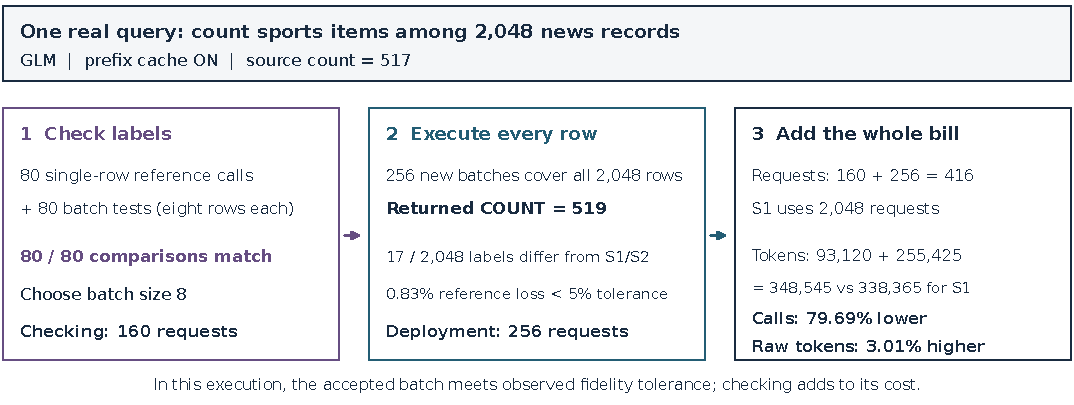
\includegraphics[width=\textwidth]{contract_execution_overview.pdf}
\caption{From a semantic COUNT query to a checked execution. The prepared review relation is the input to both checking and deployment. (a) The current-input check uses a Clopper--Pearson (CP) bound and compares one focal row per independently sampled probe batch with a singleton label. Its nominal certificate concerns agreement under that sampler. (b) Deployment labels every row once in disjoint batches, then computes COUNT outside the model. (c) We separately measure Boolean delivery and strict format, agreement with two complete singleton executions (S1/S2), COUNT error relative to the supplied-source count ($G=\sum_i g_i$), and the complete policy bill. The drawing is schematic; custom batching changes the prompt and output contract.}
\label{fig:execution}
\end{figure*}

These mechanisms have established precedents. Company studies context interference, aggregate masking of row changes and cached singleton prefixes~\cite{company}; Hassanzadeh and Subramanian measure semantic-query replay variation and cascade calibration~\cite{runvariance}. LOTUS defines optimization relative to reference algorithms~\cite{lotus}. NousDB provides the current-input fidelity check studied here and already measures calibration costs, selected sizes and efficient cached singleton execution~\cite{nousdb}. Our contribution is an empirical audit that joins the check's observations to a complete deployed result and native cost receipts in one declared engine setting. It measures how those established considerations jointly affect the plan decision.

We ask three questions:
\begin{enumerate}
\item \textbf{What is preserved?} How do delivered Booleans, strict output validity, fidelity to separate singleton executions, and COUNT accuracy against source labels differ?
\item \textbf{Does checking preserve the saving?} Do delivered batch plans stay within 5\% row disagreement with each reference while reducing complete requests and raw input-plus-output tokens? What changes with a larger checking budget?
\item \textbf{Which cost measure orders the plans?} Do raw input and native uncached-input counters favor the same plan when prefix caching is enabled?
\end{enumerate}

We execute native LOTUS filtering and deterministic COUNT with a custom multirow operator. The 36-configuration matrix spans six workloads, two domains and 512--7,600 rows using Qwen3-4B-Instruct-2507 (Qwen) and GLM-4-9B-Chat (GLM). Twelve primary configurations compare every workload at a common size/cache setting; 24 anchors vary size or cache. Sixteen follow-up policies compare 80/320-probe budgets. Complete singleton replays, deployed partitions and native receipts connect checking to results and costs.

Unchecked random and similarity batches meet the joint criterion in 1/12 and 2/12 primary configurations; the checked policy meets it in 0/12. Its sole accepted deployment preserves both observed references, but calibration consumes its raw-token saving. Larger follow-up budgets retain fallback at higher cost. Cache-enabled fixed plans favor batching on raw input and singleton execution on uncached input. Classical COUNT controls and earlier experiments place these representation-specific observations in context. The artifact preserves every configuration, negative case and resource record.\footnote{\raggedright Public materials: \url{https://github.com/yzd2002/semantic-aggregation-audit-icde2027}.}
